\documentclass{article}
\usepackage[margin=1.125in]{geometry}
\usepackage{graphicx}
\usepackage{float}
\usepackage{amsfonts}

\begin{document}
\section{Introduction} 
\textbf{Understanding the low energy behavior of the cuprate superconductors has been an open question in theoretical condensed matter physics for over thirty years.}
The cuprate materials all share a similar structure of repeating layers of square lattice CuO$_2$ planes and charge reservoir blocks, of which carriers on the prior exhibit the most interesting collective behavior. 
At zero doping the cuprates are antiferromagnetic charge-transfer insulators \cite{RevModPhys.78.17}. 
The theoretical challenge arises away from zero doping where the poorly understood superconducting, pseudo-gap, and strange metal phases appear \cite{RevModPhys.84.1383}. 
\ref{fig1} shows the phase diagram of hole- and electron-doped cuprate materials with different structures. 
The superconducting phase is d-wave in character and cannot be described by phonon-induced pairings \cite{PhysRevLett.71.2134,PhysRevLett.69.1431,PhysRevB.43.2778, PhysRevB.47.11314, PhysRevLett.70.1553, RevModPhys.67.515, RevModPhys.77.109, RevModPhys.79.353, RevModPhys.75.473}. 
In the pseudo-gap phase the d-wave gap from the superconducting state continues to partially exist, so that parts of the Fermi surface are gapped above the superconducting transition temperature \cite{ROSSATMIGNOD199186, RevModPhys.77.721, PhysRevLett.75.4114, PhysRevB.61.9752}.
The strange metal phase in the hole doped cuprates is metallic but has a "strange" resistivity which does not depend quadratically on temperature like normal Fermi liquids \cite{PhysRevLett.69.2975}, but does have T-quadratic resitivity for the electron-doped materials \cite{1989PhyC..161..415T}. 

\textbf{The strong coupling between magnetic, charge, and lattice degrees of freedom in the cuprates makes writing down a compact and accurate low energy effective theory which can describe the breadth of phenomenon related to these degrees of freedom very challenging.}
As an example of strong coupling, consider the structural phase transitions in cuprates which accompany the superconducting transition.
In La$_{2-x}$Ba$_x$CuO$_4$ (LBCO) structural phase transitions occur as doping and temperature are varied between a high temperature tetragonal phase (HTT), a low-temperature orthorhombic phase (LTO) and a low temperature tetragonal phase (LTT), and the fraction of the bulk transformed material from LTO to LTT is correlated with the bulk superconducting temperature under various dopings \cite{PhysRevLett.62.2751}. 
An independent study shows that in La$_{2-x}$Sr$_x$CuO$_{4-\delta}$ (LSCO) the superconducting phase transition for x $<$ 0.19 is accompanied by a structural phase transition from the HTT to LTO phase \cite{PhysRevB.35.7191}. 
Similarly, changes in magnetic phases and properties appear to be correlated with the superconducting phase, again providing evidence for strong coupling of microscopic degrees of freedom.
For example, there is evidence for a static stripe phase, where antiferromagnetic stripes of copper spins are separated by periodically spaced domain walls to which the holes segregate, in La$_{1.6-x}$Nd$_{0.4}$Sr$_x$CuO$_4$ at x=0.12 which is associated with an anomalous suppression in the superconducting temperature \cite{Tranquada1995, PhysRevB.54.7489}. 
Elastic magnetic measurements on La$_2$CuO$_{4+y}$ show the superconducting phase is accompanied by a spin-density wave emergence indicating a strong correlation between the two phases \cite{PhysRevB.60.3643}. 
In the undoped phase of the cuprates the magnetic dispersion across the magnetic Brillouin zone strongly resembles that of spin-waves in a square Heisenberg antiferromagnet \cite{PhysRevLett.104.077002, PhysRevLett.102.167401, PhysRevLett.105.157006}, however within the superconducting phase the magnetic dispersion takes on an "hourglass" shape which has been reproduced in experiments for LSCO at x=0.10, 0.16 \cite{PhysRevLett.93.147002}, LBCO at x=0.125 \cite{Tranquada2004}, and YBa$_2$Cu$_3$O$_{6+x}$ at x=0.5, 0.6 \cite{PhysRevB.71.024522, Hayden2004}. 
These experiments indicate that in order to write down a low-energy model for the cuprates, one has to generate effective degrees of freedom and interactions which are complicated combinations of the microscopic lattice, charge, and spin degrees of freedom.
The strong coupling between the microscopic degrees of freedom indicate that these combinations cannot be approached in a perturbative fashion from either the weak or very-strong coupling limit.

\textbf{Various models have been proposed and studied as candidates for effective theories of the cuprates, however these models were neither developed nor validated in a systematic way.}
For the undoped cuprates a nearest neighbor Heisenberg model can reproduce the magnetic dispersions measured in inelastic neutron scattering experiments accurately away from the magnetic Brillouin zone boundary, but fail to capture the small effects of anomalous dispersion near the boundary \cite{PhysRevB.79.155114, PhysRevLett.75.553}. 
The simplest model for the hole-doped cuprates was suggested by Anderson and is a 2D single-band Hubbard model which only includes bands of Cu d$_{x^2-y^2}$ character, which will be hybridized with the oxygen bands to some degree. 
In the strong coupling limit at half filling and T=0 this model reduces to a nearest neighbor Heisenberg model with long-range AFM order \cite{doi:10.1139/p78-120, PhysRevB.38.316}.
The model even exhibits a pseudo-gap like phase in the underdoped region \cite{PhysRevLett.94.156404,PhysRevB.74.024508}. 
Further, numerical studies on the Hubbard model show the existence of a $d_{x^2-y^2}$ superconducting-like phase \cite{PhysRevB.81.224505, PhysRevB.70.054504}. 
A similar model is the t-J model  which is built on the idea that under doping there are itinerant holes which hop around the oxygen bands alongside the fixed S=1/2 moments on the copper sites which interact through a superexchange term with parameter J. 
The t-J model can be seen as an effective theory of the single band t-U model. 
This model exhibits superconductivity at J/t $\sim$ 3 with a density of $\langle n \rangle$ = 1/2 \cite{PhysRevB.45.5744, PhysRevLett.70.682}.
While these models have fewer degrees of freedom and thus allow for quick numerical computations, it has been shown in accurate \textit{ab initio} Quantum Monte Carlo calculations that holes move to the oxygen bands under doping, indicating that an effective theory should include the oxygen bands explicitly, not implicity via hybridization. 
This leads to a 2D 3-band Hubbard model which includes the Cu 3$d_{x^2-y^2}$ and O p bands \cite{PhysRevLett.58.2794, VARMA1987681} and exhibits qualitatively similar behavior to the 1-band model. 
However, these approaches to generating a low-energy model have multiple issues.
First, generating the model - specifically the effective degrees of freedom, interactions and model parameters - was not done systematically, rather the choice of effective model was \textit{ad hoc}.
Second, there is no standard measure of effectiveness of the models under question. 
Typically, just a few qualitative and quantitative features of the model are compared to reality as a form of validation.

\textbf{We propose that a density matrix downfolding (DMD) \cite{10.3389/fphy.2018.00043, doi:10.1063/1.4927664} technique using \textit{ab initio} quantum Monte Carlo calculations (QMC) can systematically generate an effective model that accurately describes the low-energy properties of cuprate materials, which we will test on the electron-doped cuprate SrCuO$_2$ at T=0 and x=0, 0.125, 0.25. }
We choose to study the electron-doped cuprates because while they do not exhibit the exact same features as the hole-doped materials, they do have AFM,  superconducting, and pseudo-gap phases.
Further, the electron-doped materials have fewer relevant degrees of freedom, as electrons added to the x=0 CuO$_2$ plane can only fall into the unoccupied Cu 3d orbitals, allowing us to ignore the explicit inclusion of O p bands in our study. 
The choice of x=0, 0.125 and 0.25 at T=0 allows us to probe the most robust parts of the AFM, superconducting and metallic phases respectively, ignoring any thermal fluctuations or phase transitions like the LTO to LTT transition described earlier. 
In order to reduce the computational cost we look at the infinite-layer materials which have unit cells with the fewest number of electrons within the cuprate family.
The DMD approach allows us to map in a systematic way the \textit{ab initio} Hamiltonian to an effective model Hamiltonian, with specified model parameters and basis elements, while ensuring the model accurately reproduces the expectation value of the \textit{ab initio} Hamiltonian for states in a low-energy subspace of the full Hilbert space. 
The DMD approach also has a validation procedure which allows us to assess the effectiveness of the low-energy model in a standardized way.
In order to conduct the DMD procedure we require states in the low-energy subspace of the full \textit{ab initio} Hilbert space, which will be sampled using fixed-node diffusion Monte Carlo, a QMC algorithm which can project out low-energy states starting with appropriate trial wave functions \cite{RevModPhys.73.33}.
 
\textbf{The density matrix downfolding method (DMD) allows us to downfold a first-principles Hamiltonian into a low-energy effective theory by mapping the downfolding problem to a linear regression problem which uses ab-initio energies and reduced density matrices of wave functions sampled from a low-energy subspace of the full Hilbert space \cite{10.3389/fphy.2018.00043}. }
Consider a Hamiltonian H which acts on vectors in a Hilbert space $\mathcal{H}$ and a subset of the Hilbert space $\mathcal{LE}$ which is spanned by the lowest N energy eigenvectors of H. 
We would like to write down an effective Hamiltonian operator which acts on vectors in $\mathcal{LE}$ such that  $$\forall |\Psi\rangle \in \mathcal{LE}, H_{eff}|\Psi \rangle = H|\Psi \rangle.$$ 
It can be shown that this statement is equivalent to requiring that $$ E[\Psi] = E_{eff}[\Psi] + C \forall \Psi \in \mathcal{LE}$$ where we define the functional as $E[\Psi] = \frac{\langle \Psi | H | \Psi \rangle}{\langle \Psi | \Psi \rangle},E_{eff}[\Psi] = \frac{\langle \Psi | H_{eff} | \Psi \rangle}{\langle \Psi | \Psi \rangle}$. 
The obvious choice that would satisfy these constraints would simply be $H_{eff} = \sum_{i=1}^{N} E_i |\Psi_i\rangle \langle \Psi_i|$, but this would require us to be able to solve for the eigenstates and eigenvalues of the many-body Hamiltonian H, which we presumably cannot do. 
Instead, we may expand the $E_{eff}$ in terms of descriptors $d_i[\Psi]$ which much be chosen, simplifying the expression to just 
\begin{equation}
E_{eff} \sim \sum f_i d_i[\Psi].
\end{equation}
Now the task of generating an $E_{eff}$ that can satisfy the conditions outlined above can be cast into a statistical learning form.
Generally we will begin the DMD procedure by generating low energy states $\Psi_i$ within the space $\mathcal{LE}$. 
Additionally, we need to generate a set of descriptors $d_j$. 
Typically these descriptors take the form of expectation values of 1- or 2-rdm elements, such as $\langle \Psi| c^\dagger_k c_k |\Psi \rangle$ but can generally be any functional of $\Psi$. 
We can then use the sample states $\Psi_i$ to calculate the set of quantities $d_j[\Psi_i], E[\Psi_i]$. 
The next step is to assess whether the set of descriptors we chose and the set of states sampled are complete or not. 
For example, we might find that we have two states $\Psi_1, \Psi_2$ which have very similar descriptor values but very different energies (within the low-energy space), then it is clear that our descriptor set does not capture the variation of the energy within the space $\mathcal{LE}$ and a different descriptor must be included. 
If instead we find that we have many low-energy states with very similar energies and descriptor sets then our sampling of the low-energy space may be incomplete as we are not capturing the full variation of the descriptors we are interested in. 
In either case we may have to return to the low-energy state sampling or descriptor choosing step until we are satisfied. Once we have all of our low-energy states and important descriptors, we can simply conduct a linear regression to fit the optimal coefficients $f_j^*$ by minimizing a mean-square error (MSE) cost function:
\begin{equation}
f^{*} = argmin \Big[ \sum_{i=1}^{N} ( E[\Psi_i] - \sum_j f_j d_j[\Psi_i])^2  \Big],
\end{equation}
although other fitting approaches such as a LASSO fit can also be used \cite{10.2307/2346178}.
The $R^2$ of the fit can be used to validate the fit if using the MSE cost function, whereas different measures of goodness-of-fit are appropriate for other cost functions.
\ref{fig2} shows the workflow of the DMD procedure.
Insofar each wave function provides one data point for linear regression, however if we parameterize the wave function $\Psi_i(\vec{p})$, where $\vec{p}$ are some parameters within the wave function that can be varied without moving out of $\mathcal{LE}$, then we can generate N$_p$+1 data points per wave function where N$_p$ is the number of parameters.
This is accomplished by taking a derivative of the left and right hand sides of equation (1) with respect to the parameters $p_i$, and then minimizing a cost function like:
\begin{equation}
f^{*} = argmin \Bigg[ \sum_{i=1}^{N} \Big(\sum_{p=0}^{N_p} ( E^{(p)}[\Psi_i] - \sum_j f_j d_j^{(p)}[\Psi_i])^2 \Big) \Bigg],
\end{equation}
where $E^{(0)}[\Psi] = E[\Psi], d^{(0)}[\Psi]= d[\Psi], E^{(p)}[\Psi]=\frac{\partial E[\Psi]}{\partial p_p}, d^{(p)}[\Psi]=\frac{\partial d[\Psi]}{\partial p_p}, p\in [1,N_p].$
Therefore including parameter derivatives in our fitting procedure can increase the efficiency N$_p$ fold, decreasing the number of low-energy states that need to be sampled. 
For our situation the Hamiltonian H is the \textit{ab initio} Hamiltonian 
\begin{equation}
\hat{H_{ab}} = -\frac{1}{2} \sum_i \nabla_i^2 + \sum_{i<j} \frac{1}{r_{ij}} + \sum_{i\alpha} \frac{Z_\alpha}{r_{i\alpha}} + \sum_{\alpha<\beta} \frac{Z_{\alpha}Z_{\beta}}{r_{\alpha \beta}}
\end{equation}
where $i,j$ are electron indices, $\alpha$ is a nuclear index, with a clamped nucleus approximation and psuedo-potentials for core electrons.  

\textbf{We will use fixed node diffusion Monte Carlo (FN-DMC) to generate
wave functions in our chosen low-energy subspace and to accurately calculate ab-initio energies and reduced density matrices. }
Diffusion Monte Carlo (DMC) is a quantum Monte Carlo method which projects out the ground state of a Hamiltonian given some initial trial wave function. 
Consider a trial wave function $|\psi\rangle$ and a Hamiltonian $H$ with ground state $|\phi_0\rangle$. 
We apply the projector $e^{-\tau (H-E_0)}$ as $\tau \rightarrow \infty$ to $|\psi \rangle$
\begin{equation}
\lim_{\tau \rightarrow \infty} e^{-\tau (H-E_0)} |\psi\rangle \propto \langle \phi_0|\psi\rangle |\phi_0\rangle,
\end{equation}
projecting out the ground state $|\phi_0\rangle$ of $H$ as long as the trial wave function we choose is not orthogonal to the ground state. 
The stochastic implementation involves moving samples from the trial function $\Psi_T(R)$ using the Green function $G(R, R^\prime, \tau) = \langle R | e^{-\tau(H - E_T)} | R^\prime \rangle$. 
Since the Hamiltonian has two parts, $H = T + V$ a Trotter expansion is used to approximate the Green function $G(R, R^\prime, \tau) = \langle R | e^{-\tau(H - E_T)} | R^\prime \rangle \sim e^{-\tau(V(R) + V(R^\prime))/2} \langle R| e^{-\tau(T - E_T)}|R^\prime \rangle + O(\tau^2) $ which leads to a time step error in the calculation if the time step between moves $\tau$ is too large. 
This implementation when used on a Hamiltonian with fermions also leads to a fermion sign problem. 
We deal with this sign problem through a fixed-node approximation, where the nodal surface of the projected wave function is forced to match that of the initial trial wave function. 
This approximation makes FN-DMC variational, and will only return the exact ground state of $H$ if the nodal surfaces of $|\psi\rangle$ and $|\phi_0\rangle$ are identical. 
Therefore the FN-DMC calculation has two major systematic errors that have to be dealt with, the fixed-node error and the time-step error. 
The time-step error is typically handled through a time-step extrapolation, where multiple FN-DMC calculations are conducted at sequentially smaller $\tau$ and the relevant expectation values are extrapolated to $\tau \rightarrow 0$ \cite{Needs2010}. 
Fixed-node error can be reduced by using optimized many-body trial wave functions of the (multi-)Slater-Jastrow form seen in \cite{PhysRevLett.98.110201}.
\textbf{Need to add RDMs in DMC, mixed estimator error.}

\begin{figure}[H]
\centering
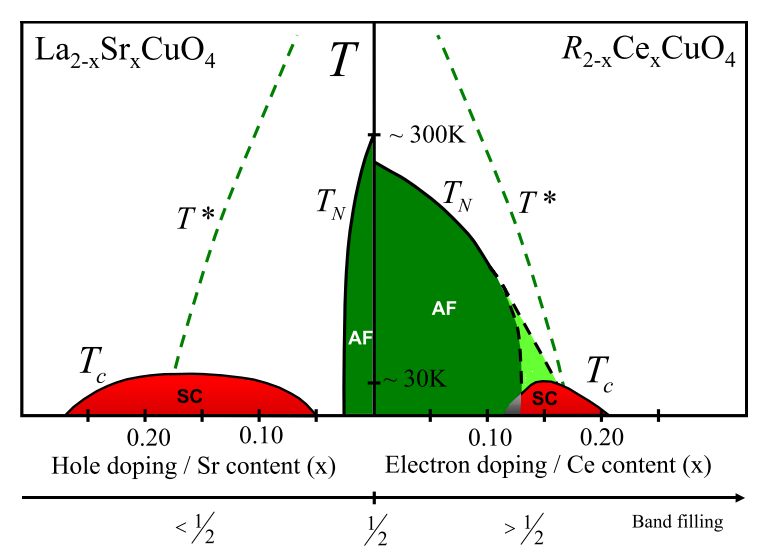
\includegraphics[width=0.6\textwidth]{Figures/I1-phase_diagram.png}
\caption{\label{fig1} Phase diagrams of the hole-doped cuprate LSCO and electron-doped cuprate family R$_{2-x}$Ce$_{x}$CuO$_4$\textit{x} and temperature \textit{T}. Figure taken from \cite{Armitage2010}. }
\end{figure}

\begin{figure}[H]
\centering
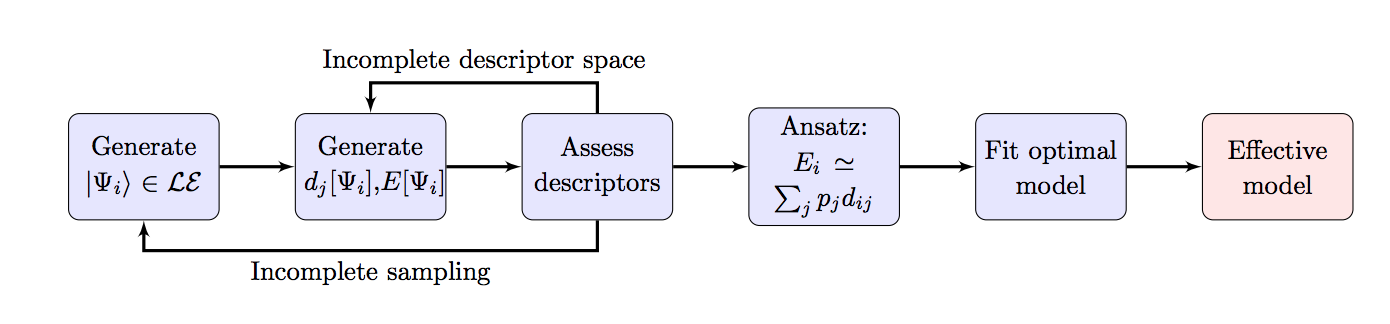
\includegraphics[width=0.9\textwidth]{Figures/I2-DMD_flow.png}
\caption{\label{fig2} Schematic drawing of the workflow for the density matrix downfolding technique, taken from \cite{10.3389/fphy.2018.00043}.}
\end{figure}

\section{Preliminary results}
In order to become acquainted with our code QWalk \cite{WAGNER20093390} and QMC algorithms in general I worked on implementing and testing multi-Slater-Jastrow trial functions with optimized non-orthogonal determinants (MSJ+NO) in FN-DMC \cite{Pathak2018}.
We assessed the efficiency and compactness of this new trial function by calculating the ground state energy and single particle densities of a C$_2$ molecule using FN-DMC and comparing to the results when using multi-Slater-Jastrow trial functions with optimized orthogonal determinant trial functions (MSJ+O). 
The workflow involved constructing the un-optimized trial wave functions, optimizing the parameters using an energy optimization method \cite{Toulouse2007}, and finally using the optimized trial functions in an FN-DMC calculation. 
We found that the FN-DMC energy calculated using an MSJ+NO trial function with only 24 determinants was lower than the FN-DMC energy using an MSJ+O trial function with 55 determinants. 
Further, the FN-DMC charge density calculated using MSJ+NO trial functions had stronger bonding character than when using MSJ+O trial functions, a reasonable result as introducing correlations into trial functions allows for electrons to avoid each other while still occupying the same bonding region. 
Our results indicated that using non-orthogonal determinants may lead to more compact multi-Slater-Jastrow trial wave functions for small molecules.

Before moving on to the computationally expensive DMD with FN-DMC calculations on SrCuO$_2$, we attempted an \textit{ad hoc} model fitting procedure using only eigenvalues and total energies from density functional theory (DFT) to get a grasp on the relevant energy scales, model terms, and values for model parameters. 
A single DFT calculation provides us three pieces of information: a Slater determinant wave function with occupied single particle orbitals $|\Psi_{DFT}\rangle$, a single particle band structure which represents the DFT eigenvalues $\epsilon(\vec{k})_{DFT}$, and a total DFT energy $E_{DFT}$. 
Suppose we have some low-energy effective model in mind with parameters $\vec{p}$, H$_m$($\vec{p}$).
We can fit the parameters in the model using only information from the DFT calculation by constructing a cost function which depends on $\vec{p}$, and then minimizing the cost. 
The cost function we used was:
\begin{equation}
Cost(w_E, \vec{p}) = \sum_{i=1}^{n} [\sum_{\vec{k}}(\epsilon(\vec{k})_{DFT,i} - \epsilon(\vec{k})_{m,i})^2] + w_E[E_{DFT,i} - \langle \Psi_{DFT,i}|H_m(\vec{p})| \Psi_{DFT,i} \rangle]^2
\end{equation}
where the sum over $i$ is over a sample of low-energy DFT states. The first term is the cost function for a least squares fit of the single particle eigenvalues calculated using our model $\epsilon(\vec{k})_m$ and the DFT state $|\Psi_{DFT,i}\rangle$ to the DFT eigenvalues. 
The second term is a cost function for a least squares fit of the total energy calculated using our model to the DFT total energy. 
The term $w_E$ controls the importance of minimizing the total energy cost relative to the eigenvalue cost, and is a variable parameter. 
The accuracy of the fit was assessed by looking at the $R^2$ value between the total energies, $R^2_E$, and between the eigenvalues, $R^2_\epsilon$. 
The fitting procedure then follows: choose a model Hamiltonian H$_m$, choose a sequence of $w_E$, minimize the cost function for each $w_E$ in the sequence and obtain a sequence of tuples $(\vec{p}, R^2_E, R^2_\epsilon)$. 
Increasing $R^2_E$ to near 1.0 will lead to a decrease in $R^2_\epsilon$ and vice versa, so the optimal model parameters are chosen by conducting a Pareto efficiency analysis on the sequence of pairs $(R^2_E, R^2_\epsilon)$. 
The Pareto optimal pair then gives us the optimal parameters $\vec{p}^\star$. 
Note that the resulting fitted effective model will not accurately reproduce the low-energy features of the \textit{ab initio} Hamiltonian H, but rather will reproduce the low-energy features of the effective Kohn-Sham theory used in our DFT calculation.

We conducted this \textit{ad hoc} fitting procedure for SrCuO$_2$ under three different dopings x=0, 0.125, and 0.25 using the PBE0 functional in DFT on a 2$\sqrt{2}$x2$\sqrt{2}$x1 unit cell. 
The PBE0 functional has been used within QMC in the past to yield accurate results for low-energy properties and energies on the hole-doped cuprates \cite{Wagner2015,Narayan2017,Wagner2014}. 
The eight unit cell calculation was chosen since it is small enough to be computationally feasible even when moving to QMC, but large enough that the finite size effects are not too large. 
For the undoped calculations, the PBE0 ground state was a checkerboard AFM state, and the six low-energy states we considered were states with spins flipped relative to this ground state. 
This choice was made since the lowest energy excitations of the undoped cuprates are spin excitations as they are charge-transfer insulators. 
For the x=0.125 calculations, the PBE0 ground state was a flip state, and the four low-energy states we considered were states with total energy less than 0.25 eV above this ground state. 
One excited state in this energy range was discarded because it was insulating in character while the other four were metallic. 
This may have occured since PBE0 has been shown to incorrectly order states energetically for strongly correlated systems.
For the x=0.25 calculations, the PBE0 ground state was a collinear state, and the four low-energy states we chose were states with total energy less than 0.30 eV above this ground state. 
Again one state in this range was insulating, while the other four were metallic, and this state was discarded from the fitting procedure. 
The model we chose to fit has four terms: 
\begin{equation}
H_m = -t \sum_{\langle i,j \rangle} c_i^\dagger c_j + h.c.
+ t^\prime\sum_{\langle \langle i.j \rangle \rangle} c_i^\dagger c_j + h.c. +\\
K\sum_{\langle i,j \rangle} \vec{S_i} \cdot c_{j,\alpha}^\dagger \vec{\sigma}_{\alpha,\beta} c_{i,\beta} + J \sum_{\langle i,j \rangle} \vec{S_i} \cdot \vec{S_j}.
\end{equation}
The operators $\vec{S_i}$ represent the spin moment on the copper sites and $c_i^\dagger$ the itinerant electrons hopping around copper sites. 
The last term is a Heisenberg exchange which we included since the undoped material can be modeled fairly accurately with just a nearest neighbor Heisenberg model with J = 0.18 eV \cite{Wagner2014}. 
The first two terms are nearest neighbor and next-nearest neighbor hopping which are both required to capture the curvature of the PBE0 bands crossing the Fermi level for the x=0.125 and x=0.25 low-energy states. 
The third term is a nearest neighbor Kondo term which we included since it can help stabilize a flip state over a checkerboard state, as seen in the x=0.125 PBE0 calculations. 
In order to extract the band structure and total energy from this model we made a mean field approximation where we split the electrons into two groups: those which contribute to the fixed spin moments $\vec{S_i}$ on site and those which are itinerant $c_i^\dagger$. 
This choice was motivated by looking at the PBE0 band structures of the low-energy states. 
As shown in \ref{fig3} the band structure is split by a large gap on the order of 1 eV, in this case for the collinear x=0.25 state. 
The bands above this gap cross the Fermi level, and can be thought of as bands which contribute only itinerant electrons. 
The bands below this gap never cross the Fermi level, and can be thought of as bands which contribute only to the fixed spin moments on copper sites. 
Therefore we can treat the quantities $\vec{S_i}$ as fixed variables, the values of which are dictated by the bands below the gap for a given PBE0 calculation. 
In doing so, the Kondo term becomes a 1-body term and the Heinsenberg term becomes a constant value, leaving the model Hamiltonian as a 1-body Hamiltonian which we can exactly diagonalize to get the total energy and eigenvalues. 

We find that the four term model above can accurately describe the PBE0 band structures and total energies of low-energy states of SrCuO$_2$ for x=0, 0.125, and 0.25. 
\ref{fig4} shows the results of our \textit{ad hoc} fitting procedure. For the undoped calculation no fitting to eigenvalues was necessary nor Pareto efficiency analysis since there were no itinerant electrons, leading to an optimal fit of $t=t^\prime=K=0 eV; J = 0.18 eV$. 
For the doped calculations, we held J fixed at the undoped value. 
This choice was made since doping with just one or two electrons in the unit cell means that most nearest neighbor copper atoms will not see the presence of the itinerant electron permanently, meaning that the local exchange interaction will not be too strongly affected.
Computationally, holding the value of J fixed at some prior made the minimization of the cost function much more stable. 
For the doped calculations, the first inset figure shows the Pareto plot with the sequence of $(R^2_E, R^2_\epsilon)$, and the Pareto optimal pair as a blue square. 
The other five insets show the fits to the bands and total energies from DFT using our model with the Pareto optimal parameters. 
For the x=0.125 calculation the optimal parameters were with $t,t^\prime,K,J$=1.15, 0.39, -0.29, 0.18 eV $R^2_E$=0.98 and $R^2_\epsilon$=0.96. 
For the x=0.25 calculation the optimal parameters were $t,t^\prime,K,J$=1.04, 0.53, -0.15, 0.18 eV with $R^2_E$=0.91 and $R^2_\epsilon$=0.94. 
In both our model and PBE0, the bands which cross the Fermi level are antibonding Cu 3d$_{x^2-y^2}$ orbitals which have been relaxed via small contributions from nearest neighbor oxygen p orbitals. 
In PBE0 the net spin moments comprised of the bands below the Fermi level also reside on the Cu 3d$_{x^2-y^2}$ orbital, indicating that unlike the hole-doped cuprates where oxygen and copper orbitals both play an important role in the effective theories, the electron-doped cuprates may be simpler since the major players is just the Cu 3d$_{x^2-y^2}$ orbital. 
Therefore the fact that $t, t^\prime$ have the same sign makes sense as this is a feature arising from the symmetry of the 3d$_{x^2-y^2}$ orbital. 
The positive sign of $J$ indicates a preference of nearest neighbor spin moments to be anti-ferromagnetically aligned, whereas the negative sign of $K$ shows a preference for itinerant electrons to ferromagnetically align with nearby spin moments. 
The opposite signs of J and K, and the fact that K is larger in magnitude than J when x=0.125 can lead to the stabilization of a flip state instead of a checkerboard one in PBE0. 

Our first step into DMD with FN-DMC was the generation of appropriate basis elements for our effective model Hamiltonian which we handled for all three dopings using intrinsic atomic orbitals. 
The \textit{ad hoc} fitting procedure we conducted provided us with a starting point for generating low-energy states for the DMD calculation, the terms in our model Hamiltonian, and parameter values, but gave us no headway on understanding which basis elements to use.
Using MOs in our model is not feasible because the interactions we are looking at are local and are nearest neighbor spatially. 
If our interaction terms were more easily written in a momentum representation then MOs from PBE0 would be a useful basis to use. 
We could start with atomic orbitals, AOs, which are the building blocks of the MOs in our PBE0 calculation, but AOs in general are not orthogonal to each other. 
This complicates our model representation because we typically work with models where creation and annihilation operators generate orthogonal states. 
Therefore, what we are looking for are orbitals that are maximally localized and still orthogonal to one another, and this is precisely what the IAO is \cite{doi:10.1021/ct400687b}. 
In order to test whether the IAO basis is sufficient at spanning the space of excitations we are interested in, we looked at the 1-body reduced density matrix (1RDM) relative to the IAO basis for each x=0, 0.125 and 0.25 low-energy state chosen above. 
We found that the total number of electrons in the system is accounted for up to three decimal places using just the trace of the 1RDM over the minimal IAO basis. 
Further, we found that the primary variation between low energy states at a fixed doping was in occupation of the IAOs was of the 3$d_{x^2-y^2}$ IAO. 
For the undoped calculations the only variation in IAO occupation among the various states was the relative occupation of the spin-up or spin-down 3$d_{x^2-y^2}$ orbital on particular copper sites. 
This makes sense as the only difference between the undoped low-energy states was the configuration of local spin moments. 
Under doping, the primary variation in orbital occupation was found in the 3$d_{x^2-y^2}$ IAO which had the lower occupancy.
This makes sense as the only place the added electron can go is in the 3$d_{x^2-y^2}$ orbital in the spin channel opposite to the local moment on the site. 
\ref{fig5} shows the IAOs for the majority spin IAO, which has the higher occupation, and the minority spin IAO, which has the lower spin, for a low-energy state at x=0.125. 
It is clear that the majority spin IAO is more tightly localized on site whereas the minority spin IAO spreads across the unit cell with contributions from oxygen p-orbitals. 
We therefore come to the conclusion that the majority spin IAOs should be used as a basis for the localized spin moments, $\vec{S_i}$, and the minority spin IAOs should be used as a basis for the itinerant electrons, $c_i^\dagger$. 

\begin{figure}[H]
\centering
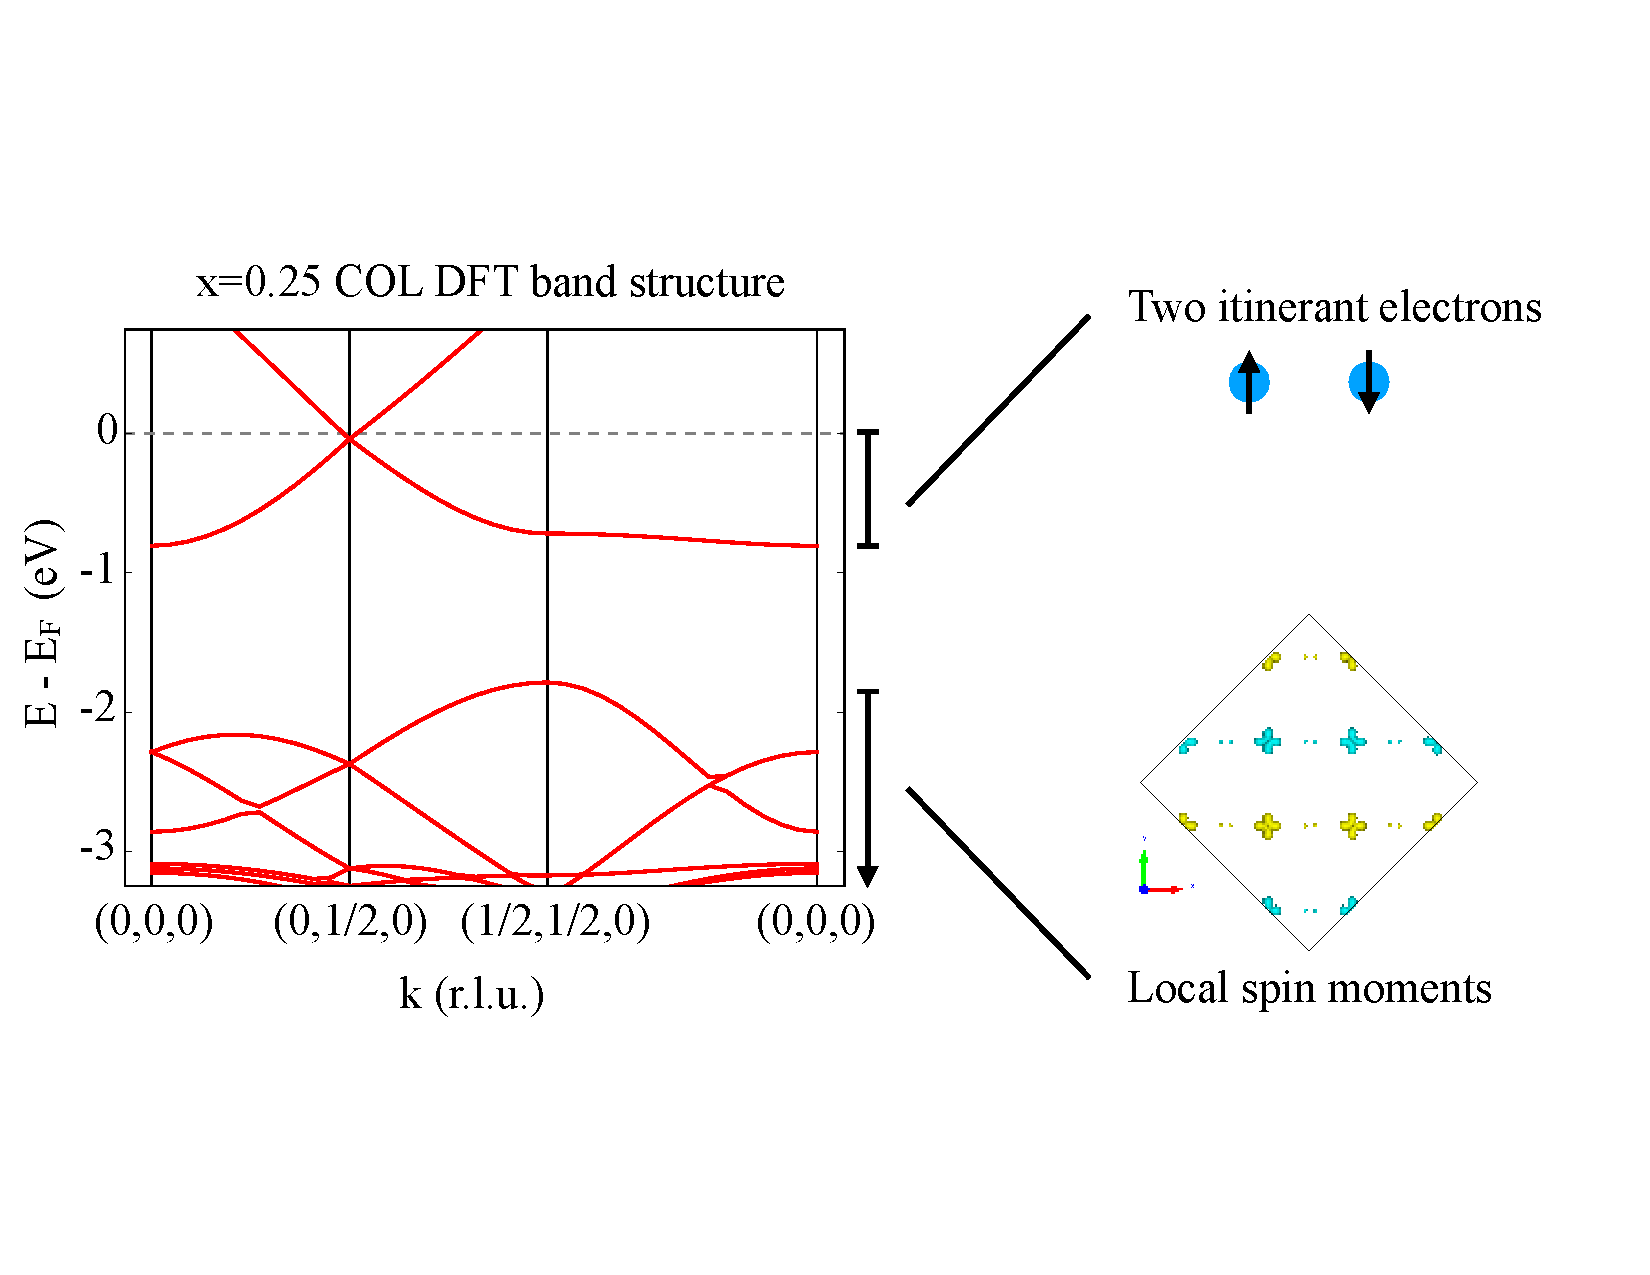
\includegraphics[width=0.6\textwidth]{Figures/R1-mean_field.pdf}
\caption{\label{fig3} Schematic diagram showing the method for mean-field approximation we used in our DFT model fitting calculations.}
\end{figure}

\begin{figure}[H]
\centering
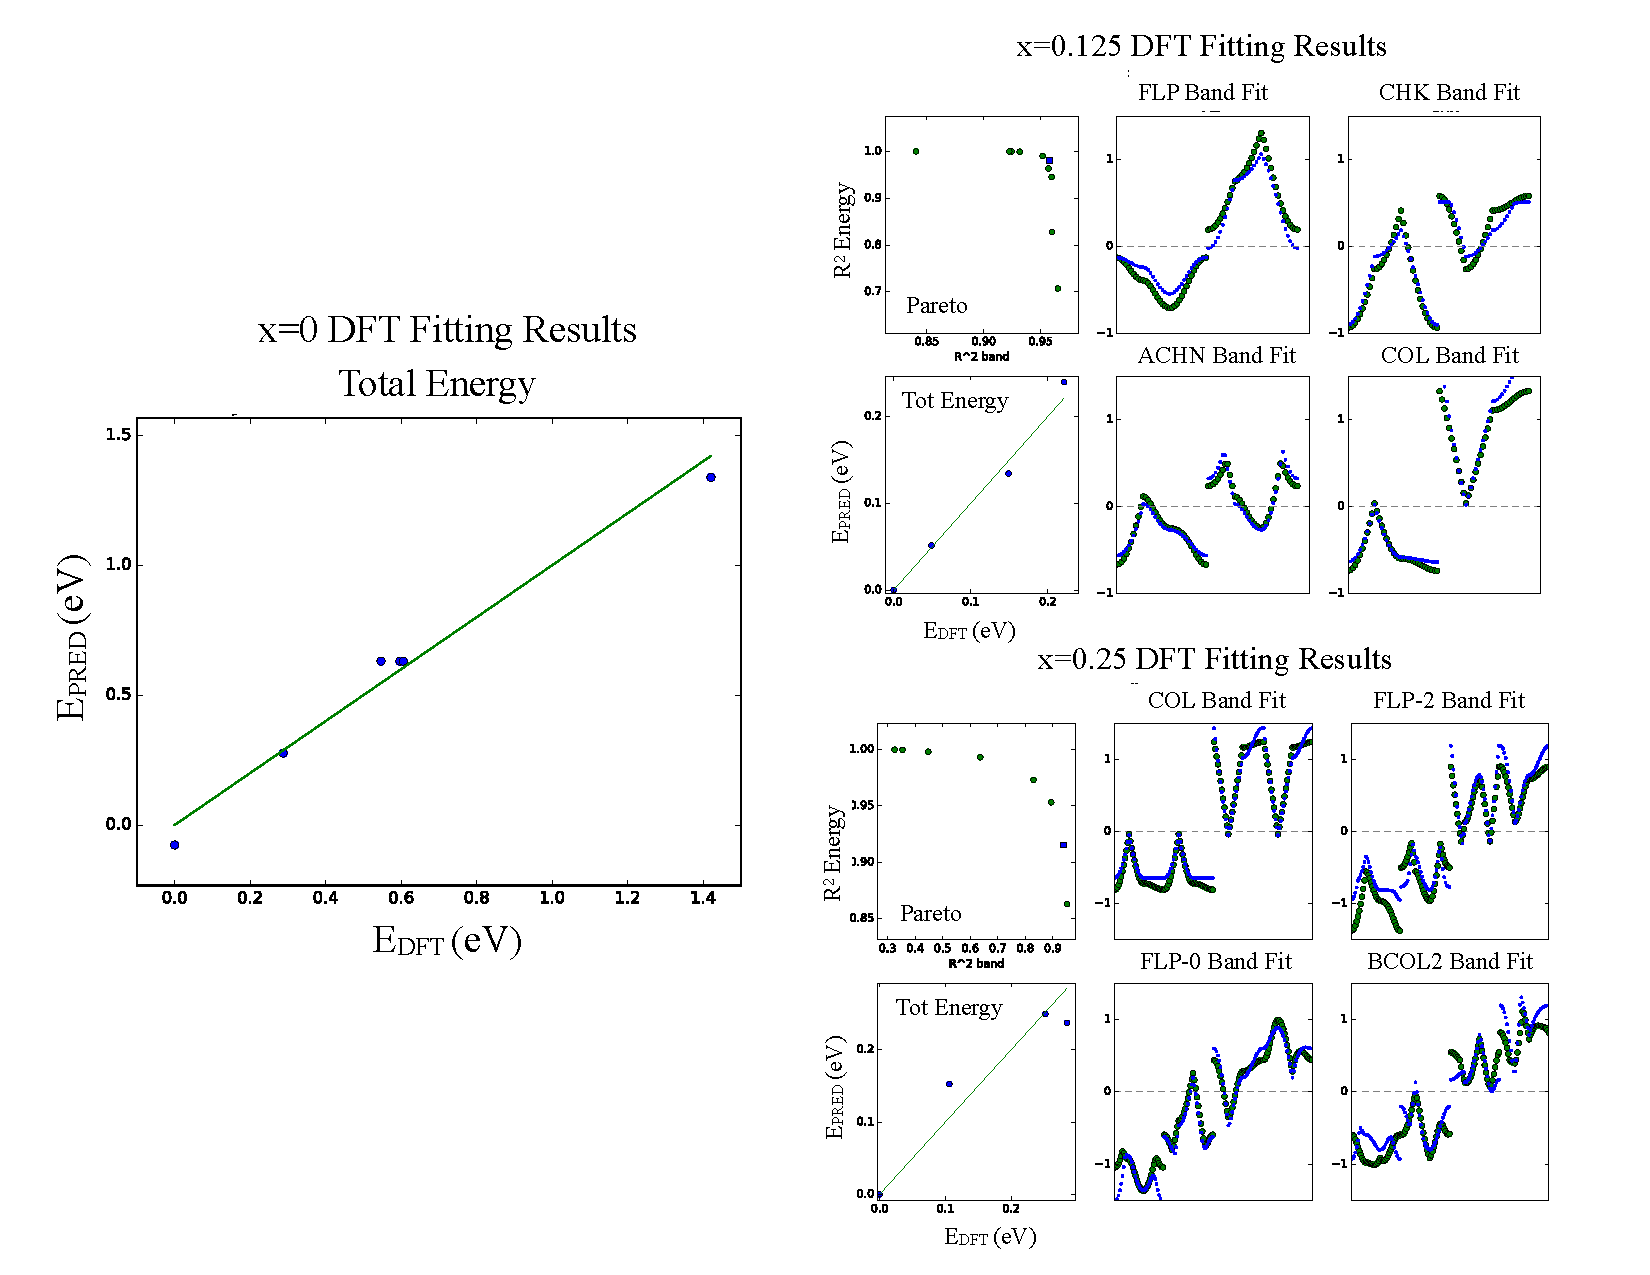
\includegraphics[width=0.9\textwidth]{Figures/R2-pareto.pdf}
\caption{\label{fig4} Results of the \textit{ad hoc} fitting procedure just using the DFT eigenvalues and total energies for three different dopings.}
\end{figure}

\begin{figure}[H]
\centering
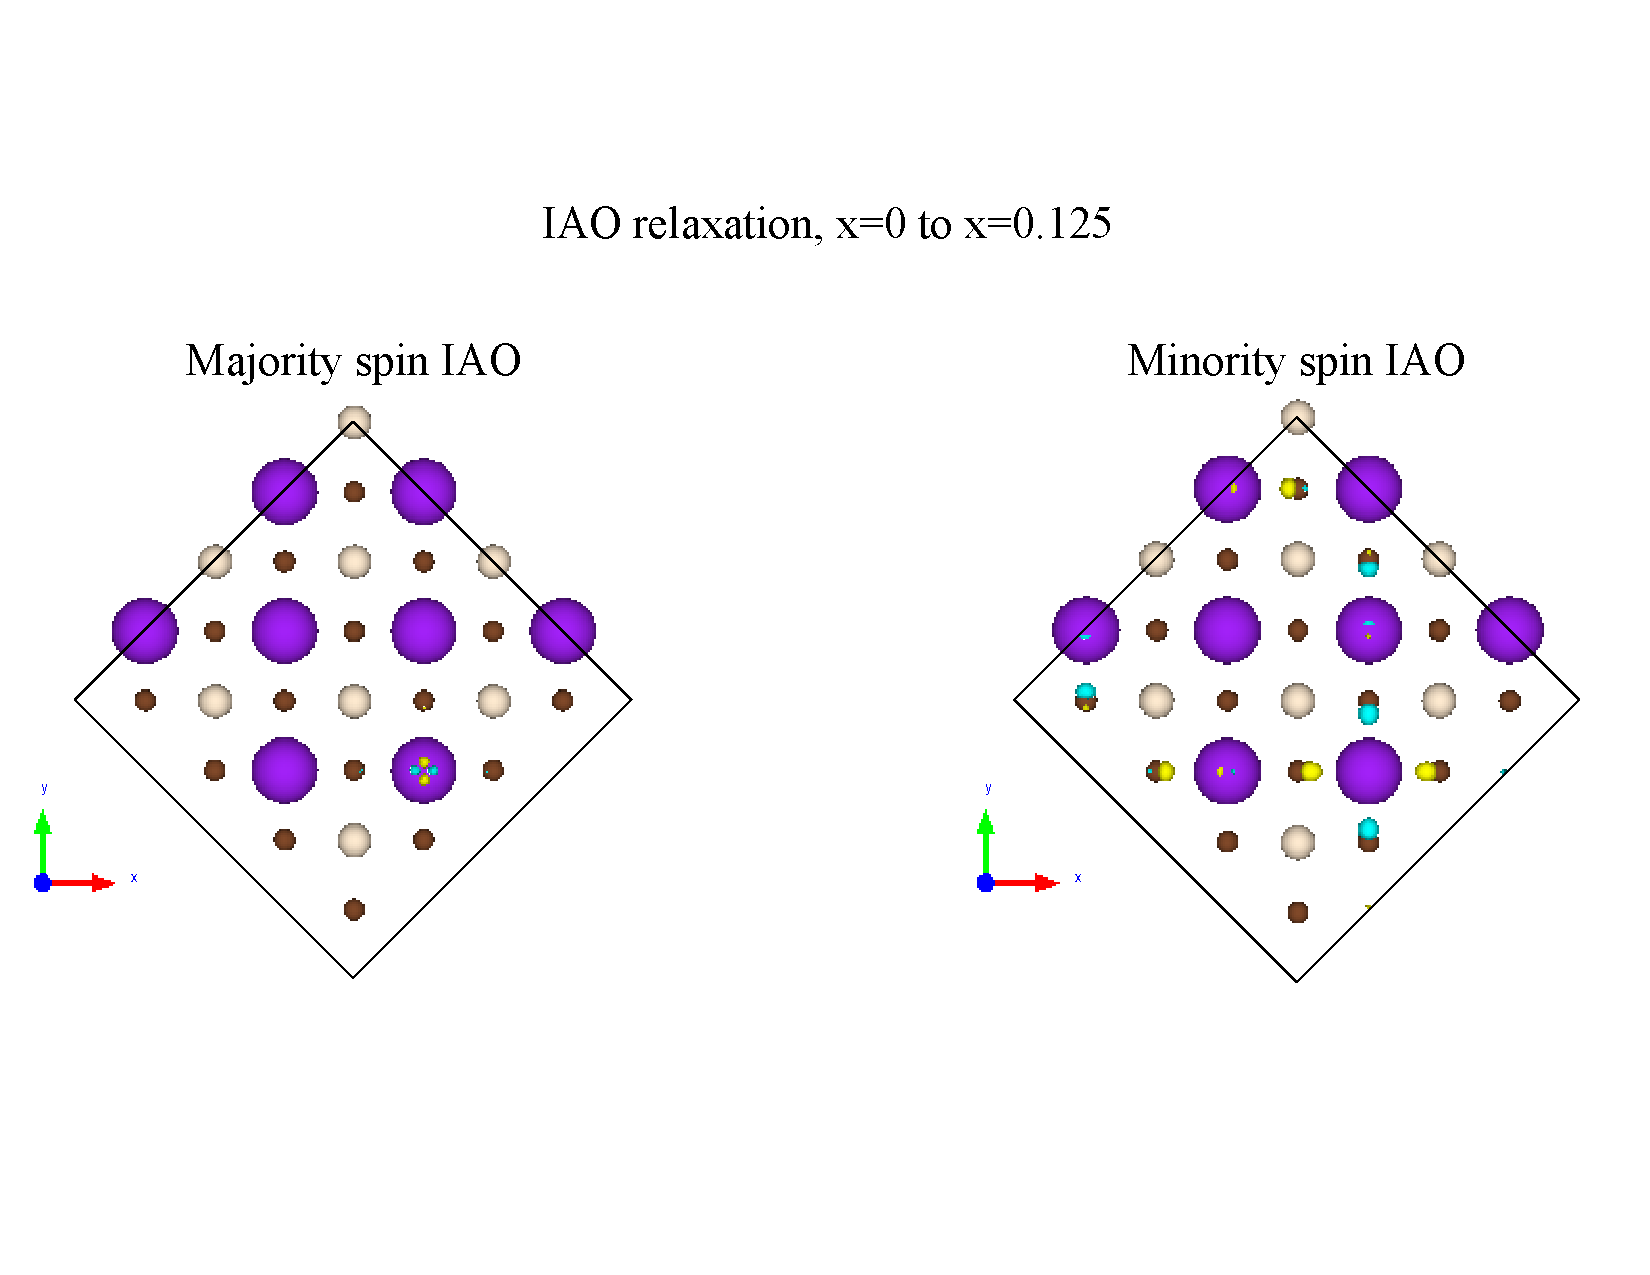
\includegraphics[width=0.9\textwidth]{Figures/R3-iao_basis.pdf}
\caption{\label{fig5} Relaxation of the IAOs for the spin majority and minority channel under doping for the eighth doped flip state. The majority spin IAO can be used as a basis for the fixed spin moments and the minority spin IAO for the itinerant electrons.}
\end{figure}
\pagebreak

\section{Proposed work}
In order to generate an effective low-energy model using the DMD technique we need to generate low-energy wave functions within the full \textit{ab initio} Hilbert space. 
We will be using optimized multi-Slater-Jastrow (MSJ) as trial wave functions in FN-DMC to generate the low-energy states we are interested in. 
The MSJ wave function form 
\begin{equation}
\Psi_{MSJ} = e^{J(\vec{\alpha})} \sum_I c_I |D_I{\{\phi\}}\rangle 
\end{equation}
has two core parts, the multi-determinant expansion with determinant coefficients $c_I$ and a 3-body Jastrow factor with some Jastrow coefficients $\alpha$. 
These parameters will be optimized using an energy optimization method described by \cite{Toulouse2007}. 
The determinants will be composed of single particle orbitals from the eight unit cell DFT calculations we have already completed.	
The multi-determinant expansion will be generated using a (complete) active space (C)AS expansion using the Cu 3d and 4s bands and the O 2p bands. 
We believe that these bands include the relevant degrees of freedom to generate an accurate low-energy model. 
The (C)AS expansion allows us to generate many low-energy states by simply varying the coefficients $\{c_I\}_{I>0}$ within some cutoff. 
After generating these trial wave functions we can use FN-DMC to project out a low-energy state within the \textit{ab initio} Hilbert space, calculate the total FN-DMC energy, 1- and 2-body reduced density matrices using the IAO basis that we have already generated, as well as derivatives of the total energy and the density matrices with respect to the determinant coefficients $c_I$. 
We will not consider derivatives with respect to the Jastrow coefficients because that derivative will take us outside of the low-energy space, as the Jastrow factor significantly reduces the total energy of a trial state \cite{PhysRevLett.75.3870}.

After the data generation phase above from which we have all the information required to do our fitting, relevant descriptors have to be chosen for our low-energy model. 
The first tool in reducing the space of relevant descriptors is through symmetry considerations. Coury \textit{et al} \cite{Coury2016} provides a useful manual for the terms that any 1- and 2-body Hamiltonian can have given the symmetry of the bands that are under consideration. 
From here we arrive at a basic statistics problem of generating a linear model given a potential set of descriptors. 
A very basic approach to solving this problem is through a greedy selection algorithm. 
This selection algorithm iteratively includes more and more descriptors to our model Hamiltonian, at each step including a term which would reduce the $R^2$ value between the \textit{ab initio} energies of our low-energy states and the model energies $\langle H_m \rangle$. 
This method does not span the space of all possible models given the symmetry constraints above, but is an efficient choice given the very large space of model Hamiltonians that could be chosen. 
The greedy selection algorithm can then take our data and generate a sequence of models with increasing complexity, provide the best values of the model parameters for each model, and also provide a measure of the fit through the $R^2$ value. 
We can then manually choose a model which has a large $R^2$ with a relatively small model complexity. 
This choice can also be made systematically by using an Akaike information criterion \cite{ref591} or Bayesian information criterion \cite{schwarz1978} to measure the goodness of fit at each step of the greedy algorithm instead of a simple least-square measure of goodness. 
These two criteria penalize a model not only for the least-square measure of goodness but also for model complexity.

Since our initial set of calculations will be on an eight unit cell calculation cell with periodic boundary conditions, it is important to account for possible finite size errors in our FN-DMC calculations. 
If these finite size errors (FSEs) are not accounted for in FN-DMC then the model we generated may suffer from the same finite size effects as the QMC calculations. 
Within QMC there are typically two approaches to dealing with finite size effects. 
To deal with finite size effects affecting single particle properties a common choice is to use twist-averaging. 
This means conducting the many-body FN-DMC calculation using various twisted boundary conditions and then averaging over the results of the single-particle expectation values \cite{Lin2001, PhysRevB.78.125106}.
This is equivalent to averaging over the many-body Brillouin zone. 
To account for two-particle or higher order finite size effects, such as those affecting the Coulomb interaction term when calculating the total energy, a finite size extrapolation is required. 
This involves conducting the FN-DMC calculations for a sequence of increasing calculation cell size, and then extrapolating the results of expectation values to the infinite cell size. 
The extrapolation scales linearly with the cell volume \cite{PhysRevB.78.125106}.

Further, we will use the DMD procedure to attempt to describe the differences between the isostructural nickelate and cuprate materials. 
Shown in \ref{fig6} are the conventional unit cells of the cuprate La$_2$CuO$_4$ and the nickelate La$_2$NiO$_4$, which are identical except that the copper atom within the cell is replaced by a nickel atom. 
While isostructural, the nickelates have been shown to not superconduct even down to temperatures of mK \cite{PhysRevB.43.1229} under doping. 
In order to study this distinct difference in low-energy behavior, we will use the DMD procedure listed above in an identical fashion on the material SrNiO$_2$. 
The relevant degrees of freedom are the same for both the nickelate and cuprate materials, meaning the active space used to generate low-energy states will be Cu 3d, 4s and O 2p for both cases. 
If we consider a slightly higher energy cutoff for our low-energy theory, it may be possible that our DMD procedure generates an effective theory with identical descriptors but different model parameters. 
The reasoning behind this argument stems from the fact that effective models like the Hubbard model can yield various low-energy effective theories when considered under certain parameter regimes, meaning that two materials can, at the lowest energy scales, have drastically different low-energy theories while at a higher energy scales be described accurately by similar effective theories. 
Having a single model which can describe the low-energy behavior of both of these materials would provide a big step forwards to understanding the emergence of superconductivity in the cuprates and the lack thereof in the nickelates. 

\begin{figure}[H]
\centering
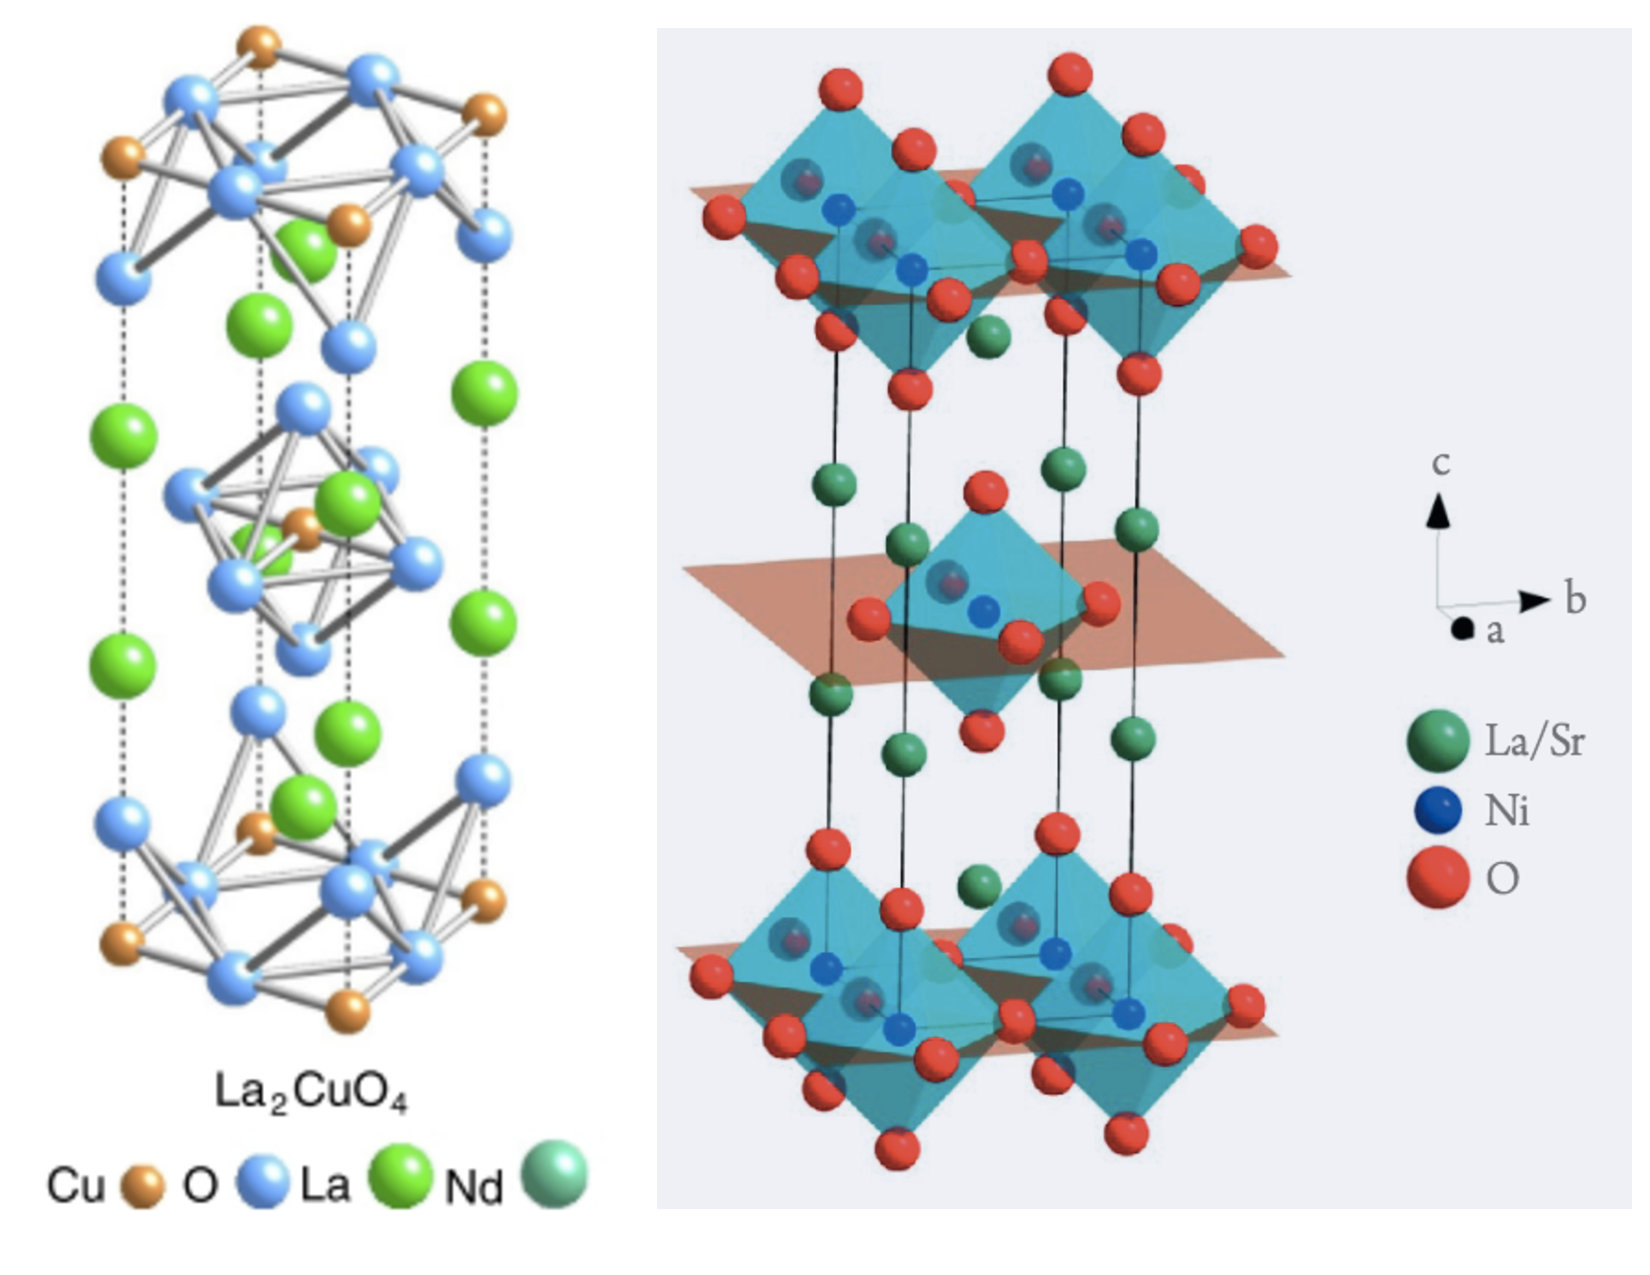
\includegraphics[width=0.9\textwidth]{Figures/P2-Ni_Cu.pdf}
\caption{\label{fig6} The primitive unit cells of the isostructural materials LNCO \cite{PhysRevB.92.205114} and LSCO \cite{Scalapino2012}, the prior which is not super conducting all the way to temperatures of 30mK.}
\end{figure}

%\section{References}
%\begin{enumerate}
%\item https://journals.aps.org/rmp/abstract/10.1103/RevModPhys.82.2421 (Figure?)

%\end{enumerate}
 
\bibliographystyle{unsrt}
\bibliography{biblio} 
 
\end{document}